\documentclass[11pt,a4paper]{article}
\author{TalentSprint}
\date{}
\usepackage{verbatim}
\usepackage{fancyhdr}           % For header and footer
\usepackage{multicol}
\usepackage{colortbl}           % For coloured tables
\usepackage{setspace}           % For line height
\usepackage{seqsplit}           % Splits long words.
\usepackage{amsmath} 
\usepackage{graphicx}
\usepackage{array}
\usepackage{enumitem}
\usepackage{xcolor}
\usepackage[tikz]{bclogo}
\usepackage{textcomp}
\usepackage{listings}
\lstset{language=python,numbers=left,numberstyle=\tiny,numbersep=10pt,showstringspaces=false}

\headheight=14pt
\lhead{\nouppercase{}}
\rhead{\nouppercase{\leftmark}}

\newcommand*\lstinputpath[1]{\lstset{inputpath=#1}}
\lstinputpath{../Code/}
\graphicspath{{../Images/} {../ScreenShots/}}

\setcounter{tocdepth}{1}
\setlength\parindent{0pt}
\parskip=4pt
\newcommand{\Code}[1]{\textbf{\texttt{#1}}}

% Lengths and widths
\addtolength{\textwidth}{5cm}
\addtolength{\hoffset}{-1cm}
\setlength{\headsep}{-12pt} % Reduce space between header and content
\setlength{\headheight}{85pt} % If less, LaTeX automatically increases it
\renewcommand{\footrulewidth}{2pt} % Remove footer line
\renewcommand{\headrulewidth}{1pt} % Remove header line
\renewcommand{\seqinsert}{\ifmmode\allowbreak\else\-\fi} % Hyphens in seqsplit
% This two commands together give roughly
% the right line height in the tables
\renewcommand{\arraystretch}{1.3}
\onehalfspacing

% Commands
\newcommand{\SetRowColor}[1]{\noalign{\gdef\RowColorName{#1}}\rowcolor{\RowColorName}} % Shortcut for row colour
\newcommand{\mymulticolumn}[3]{\multicolumn{#1}{>{\columncolor{white}}#2}{#3}} % For coloured multi-cols
\newcolumntype{x}[1]{>{\raggedright}p{#1}} % New column types for ragged-right paragraph columns
\newcommand{\tn}{\tabularnewline} % Required as custom column type in use

% Font and Colours
\definecolor{HeadBackground}{HTML}{333333}
\definecolor{FootBackground}{HTML}{666666}
\definecolor{TextColor}{HTML}{333333}
\definecolor{DarkBackground}{HTML}{6B8E23} %{FD1AA8}
\definecolor{LightBackground}{HTML}{E8FED8} %D3FDC8
\definecolor{tit}{HTML}{FF6600}
\renewcommand{\familydefault}{\sfdefault}
\color{TextColor}
 \headsep = 25pt
% Header and Footer
\pagestyle{fancy}
\usepackage[headheight=110pt]{geometry}
\fancyhf{}% Clear header/footer

\fancyhead[r]{
\includegraphics[width = 4cm, height = 2cm]{TS-Logo.png}\hspace{0cm}}

%=================================TITLE=====================================
\fancyhead[l]{\Large{\bf{\textcolor{tit}{\textrm{Command Line Arguments}}}}}
%===========================================================================

\renewcommand{\headrulewidth}{0.4pt}% Default \headrulewidth is 0.4pt
\renewcommand{\footrulewidth}{0.4pt}% Default \footrulewidth is 0pt

\rfoot{Page \thepage}
\lfoot{COPYRIGHT \textcopyright TALENTSPRINT, 2015. ALL RIGHTS RESERVED.}

\begin{document}


%\chapter{Command Line Arguments}
It is possible to pass some values from the command line to your C programs when they are executed. These values are called command line arguments and many times they are important for your program specially when you want to control your program from outside instead of hard coding those values inside the code.

\section*{Command Line Arguments}
The command line arguments are handled using \texttt{main()} function arguments. main receives two arguments from the Operating System (Shell); traditionally they are called \textbf{\texttt{argc}} and \textbf{\texttt{argv}}, though any name can be given. \texttt{argc} is an integer and refers to the number of arguments passed, and \texttt{argv[]} is a pointer array which points to each argument passed to the program as a string.

\begin{lstlisting}[numbers=none]
  int main(int argc, char* argv[]) {
\end{lstlisting}

Now argc and argv are like any variables in the program.

\begin{enumerate}
\item The \emph{main()} can and should check \texttt{argc} to see how many arguments the user specified.
\item The minimum count for \texttt{argc} is 1; in this case the \emph{argument} is just the name of the program itself.
\item Which means, a program can find out its own name as it was invoked! It is the string \texttt{argv[0]}. This is OS dependent.
\item The arguments are always strings. If you expect to receive an integer as the argument, you should convert it inside the code. 
\item Command line arguments are separated by a space, but if an argument itself has a space then you can pass such arguments by putting them inside quotes.
\end{enumerate}

\subsubsection*{Example} 

Let us start with a simple example:
\lstinputlisting{Program-12-1.c}

When the above code is compiled and executed with a single argument, it produces the following result.

\begin{figure}[ht]
\begin{center}
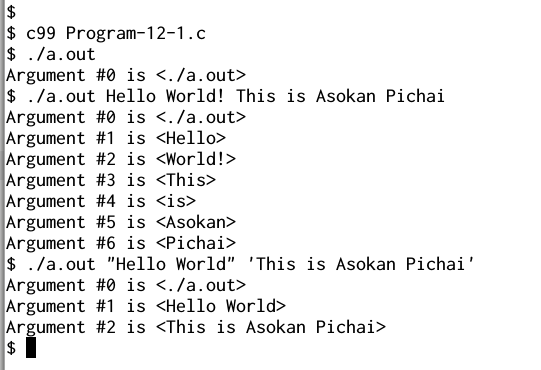
\includegraphics[scale=0.6]{Output-12-1.png}
\caption{Echoing Command line arguments}
\label{output-12-1}
\end{center}
\end{figure}

A more complicated example: let us build a command line calculator for binary expressions.

\lstinputlisting{Program-12-2.c}

\begin{figure}[ht]
\begin{center}
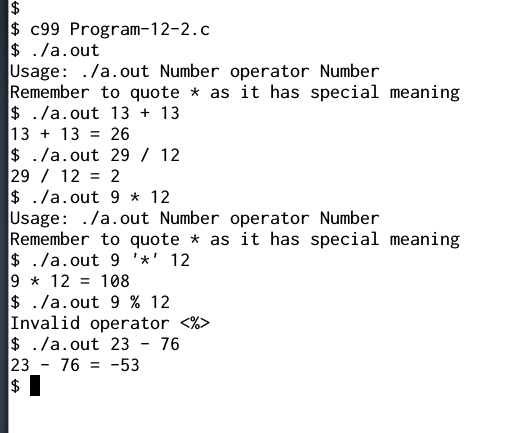
\includegraphics[scale=0.6]{Output-12-2.png}
\caption{Command line calculator}
\label{output-12-2}
\end{center}
\end{figure}

Please note that we have not validated that only integers have been entered.
\end{document}